\documentclass{article} % A4 paper and 11pt font size
\setcounter{secnumdepth}{0}

\usepackage{amssymb, amsmath, amsfonts}
\usepackage{moreverb}
\usepackage{graphicx}
\usepackage{enumerate}
\usepackage{graphics}
\usepackage[margin=1.25in]{geometry}
\usepackage{color}
\usepackage{tocloft}
\renewcommand{\cftsecleader}{\cftdotfill{\cftdotsep}}
\usepackage{array}
\usepackage{float}
\usepackage{csquotes}
\usepackage{verbatim}
\usepackage{hyperref}
\usepackage{textcomp}
\usepackage[makeroom]{cancel}
\usepackage{bbold}
\usepackage{scrextend}
\usepackage{alltt}
\usepackage{listings}
\usepackage{physics}
\usepackage{mathtools}
\usepackage[normalem]{ulem}
\usepackage{amsthm}
\usepackage{tikz}
\usetikzlibrary{positioning}
\usetikzlibrary{arrows}
\usepackage{pgfplots}
\usepackage{bigints}
\allowdisplaybreaks
\pgfplotsset{compat=1.12}

\theoremstyle{plain}
\newtheorem*{theorem*}{Theorem}
\newtheorem{theorem}{Theorem}
\newtheorem*{lemma*}{Lemma}
\newtheorem{lemma}{Lemma}

\definecolor{verbgray}{gray}{0.9}
% \definecolor{dkgreen}{green}{0.9}

\lstnewenvironment{code}{%
  \lstset{
  language=R,
  backgroundcolor=\color{verbgray},
  keywordstyle=\color{blue},      % keyword style
  commentstyle=\color{magenta},   % comment style
  stringstyle=\color{olive},      % string literal styleframe=single,
  numberstyle=\color{black},      % string literal styleframe=single,
  framerule=0pt,
  numbers=left,
  stepnumber=1,
  firstnumber=1,
  showspaces=false,
  basicstyle=\ttfamily}}{}

\lstnewenvironment{console_output}{%
  \lstset{
  framerule=0pt,
  numbers=left,
  stepnumber=1,
  showspaces=false,
  firstnumber=1,
  basicstyle=\ttfamily}}{}


\makeatletter
\newcommand{\BIGG}{\bBigg@{3}}
\newcommand{\vast}{\bBigg@{4}}
\newcommand{\Vast}{\bBigg@{5}}
\makeatother

\newenvironment{definition}[1][Definition]{\begin{trivlist}
\item[\hskip \labelsep {\bfseries #1}]}{\end{trivlist}}

\newcommand{\dy}{\partial_y}
\newcommand{\dyy}{\partial_{yy}}
\newcommand{\dxx}{\partial_{xx}}
\newcommand{\dxy}{\partial_{xy}}
\newcommand{\dyyy}{\partial_{yyy}}
\newcommand{\dxxx}{\partial_{xxx}}
\newcommand{\dx}{\partial_x}
\newcommand{\E}{\varepsilon}
\def\Rl{\mathbb{R}}
\def\Cx{\mathbb{C}}

\newcommand{\Ei}{\text{Ei}}

\usepackage[T1]{fontenc} % Use 8-bit encoding that has 256 glyphs
\usepackage{fourier} % Use the Adobe Utopia font for the document - comment this line to return to the LaTeX default
\usepackage[english]{babel} % English language/hyphenation

\usepackage{sectsty} % Allows customizing section commands
\allsectionsfont{\centering \normalfont\scshape} % Make all sections centered, the default font and small caps

\usepackage{fancyhdr} % Custom headers and footers
\pagestyle{fancy} % Makes all pages in the document conform to the custom headers and footers
\fancyhead[L]{\bf Sam Fleischer}
\fancyhead[C]{\bf UC Davis \\ Principles of Population Biology (PBG200A)} % No page header - if you want one, create it in the same way as the footers below
\fancyhead[R]{\bf Fall 2016}

\fancyfoot[L]{\bf } % Empty left footer
\fancyfoot[C]{\bf \thepage} % Empty center footer
\fancyfoot[R]{\bf } % Page numbering for right footer
\renewcommand{\headrulewidth}{0pt} % Remove header underlines
\renewcommand{\footrulewidth}{0pt} % Remove footer underlines
\setlength{\headheight}{25pt} % Customize the height of the header

\newcommand{\VEC}[2]{\left\langle #1, #2 \right\rangle}
\newcommand{\ran}{\text{\rm ran }}
\newcommand{\Hilb}{\mathcal{H}}
\newcommand{\lap}{\Delta}

\newcommand{\littleo}[1]{\text{\scriptsize$\mathcal{O}$}\qty(#1)}

\DeclareMathOperator*{\esssup}{\text{ess~sup}}

\newcommand{\problem}[2]{
\vspace{.375cm}
\boxed{\begin{minipage}{\textwidth}
    \section{\bf #1}
    #2
\end{minipage}}
}

\numberwithin{equation}{section} % Number equations within sections (i.e. 1.1, 1.2, 2.1, 2.2 instead of 1, 2, 3, 4)
\numberwithin{figure}{section} % Number figures within sections (i.e. 1.1, 1.2, 2.1, 2.2 instead of 1, 2, 3, 4)
\numberwithin{table}{section} % Number tables within sections (i.e. 1.1, 1.2, 2.1, 2.2 instead of 1, 2, 3, 4)

\setlength\parindent{0pt} % Removes all indentation from paragraphs - comment this line for an assignment with lots of text

\newcommand{\horrule}[1]{\rule{\linewidth}{#1}} % Create horizontal rule command with 1 argument of height

\title{ 
\normalfont \normalsize 
\textsc{UC Davis, Applied Mathematics (MAT207C), Spring 2016} \\ [25pt] % Your university, school and/or department name(s)
\horrule{2pt} \\[0.4cm] % Thin top horizontal rule
\Huge Homework \#8 \\ % The assignment title
\horrule{2pt} \\[0.5cm] % Thick bottom horizontal rule
}

\author{\huge Sam Fleischer} % Your name

\date{June 3, 2016} % Today's date or a custom date

\begin{document}\thispagestyle{empty}

\maketitle % Print the title

\makeatletter
\@starttoc{toc}
\makeatother

\pagebreak

%%%%%%%%%%%%%%%%%%%%%%%%%%%%%%%%%%%%%%
\problem{Problem 1}{The whooping crane has been the target of protection efforts by the National Audubon Society and the federal governments of the US and Canada since 1941. There is one wild breeding population that winters at the Arkansas National Wildlife Refuge on the coast of Texas. The size of this population from 1941 to 1989 was studied by Dennis et al. (1991) in their Ecological Monographs paper Estimation of growth and extinction parameters for endangered species. The data set used by Dennis et al. is in the cranes.csv data file in the resources folder at SmartSite.
\begin{enumerate}[\ \ (a)]
    \item Assuming the log population numbers can be modeled by
    \begin{align}
        \log N(t) = \log N(0) + rt + \text{``observation error''}
    \end{align}
    where the ``observation error'' is normally distributed, use linear regression to estimate $\log N(0)$ and $r$.  Use this model to estimate $N(2011)$.
    \item Assuming the log population numbers can be modeled by
    \begin{align}
        \log \frac{N(t+1)}{N(t)} = r + \text{``process error''}
    \end{align}
    where the ``process error'' is normally distributed, use linear regression to estimate $r$.  Use this model to estimate $N(2011)$.
    \item Do an online search to find an estimate for the \emph{wild} whooping population size in August 2011.  How do your model predictions compare?
\end{enumerate}}
\begin{enumerate}[\ \ (a)]
    \item
        The following code snippet was used to load the CSV file and run a linear regression on the log population numbers.
        \begin{code}
# Load the file
cranes = read.csv("cranes-2013.csv")

# Set local variables to access the data
Count = cranes$Count
Year = cranes$Year

# Plot Count vs. Year
plot(Year, Count, pch=4)

# Take the logarithm of the population numbers.
logPop = log(Count)

# Perform a linear regression
regression = lm(logPop~Y)

# Add the exponential (line in log-space) to the plot
lines(Year,exp(regression$fitted.values))

# Print the summary of the regression
summary(regression)
        \end{code}
        The output from the summary command shows $\log N(0) \approx -78.86$ and $r \approx 0.04204$, so $\log N(t) \approx -78.86 + 0.04204t$, which then implies
        \begin{align}
            N(t) \approx N_0\exp[0.04204t] \qquad \text{with} \qquad N_0 = \exp[-78.86].
        \end{align}
        Below is the plot generated from the code snippet.
        \begin{figure}[ht!]
            \centering
            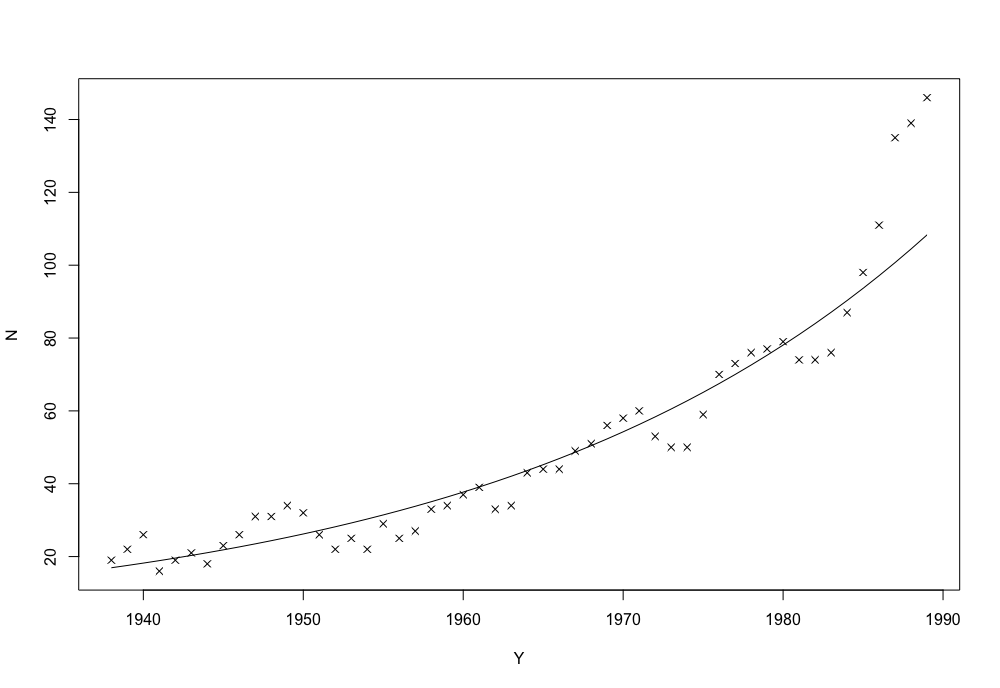
\includegraphics[scale=0.3]{1a.png}
        \end{figure}
        Using this linear regression, $N(2011) \approx 293.67$.

    \item
        The following code snippet was used to load the CSV file and run a linear regression on the ratio of successive log population numbers.
        \begin{code}
# Load the file
cranes = read.csv("cranes-2013.csv")

# Use the variable ``N'' as the population
N = cranes$Count

# Take the log of the population
logN = log(N)

# Get ``future'' and ``past'' arrays
logNtp1 = logN[-1]
logNt = logN[-length(logN)]

# Plot them against each other
plot(logNt,logNtp1)

# Linearly regress them and plot the result
regression = lm(logNtp1~logNt)
lines(logNt,regression$fitted.values)

# Print the result of the regression
summary(regression)
        \end{code}
        The output from the summary command shows $\log N_{t+1} \approx 0.99038\log N_t + 0.08309$, which implies
        \begin{align}
            N_{t+1} = e^{0.08309}N_t^{0.99038}
        \end{align}
        Using $N_{2010}$ from the data, ($N_{2010} = 281$), we get the approximation $N_{2011} = 289.22$.  Using the initial condition $N_{1955} = 29$ and the above recursive rule, we get the approximation $N_{2011} = 262.5$.

    \item
        The website {\color{blue}\hyperlink{https://www.learner.org/jnorth/tm/crane/PopulTotals.html}{https://www.learner.org/jnorth/tm/crane/PopulTotals.html}} gives the wild Whooping Crane Population in the Western Flock as 278.  It looks like the linear regression from (a) overestimated the most, while the average of the results from (b) is 275.86, which is very close to the actual value.
\end{enumerate}













%%%%%%%%%%%%%%%%%%%%%%%%%%%%%%%%%%%%%%
\problem{Problem 2}{\textbf{Monad's nightmare:} Starting with a single cell of \emph{E. coli}, how long would it take to cover the Earth 1 foot deep with \emph{E. coli}?  Assume that \emph{E. coli} are rectangular prisms of volume $1.1250\times10^{-18} \text{meters}^3$ and that they reproduce every 20 minutes.}

The radius of the Earth is approximately $20903520 \text{ feet}$, and thus the volume of the $1 \text{ foot}$ film of \emph{E. coli} around the Earth is
\begin{align}
    V_{\text{film}} = \frac{4}{3}\pi 20903521^3 - \frac{4}{3}\pi 2090352103^3 = 5490965741568000 \text{ feet}^3 \approx 155486834545908.5625 \text{ meters}^3
\end{align}
This means it would take approximately $\frac{155486834545908.5625}{1.1250\times10^{-18}} \approx 1.3821051959636316\times 10^{32}$ \emph{E. coli} cells to cover the earth with a $1$ foot film.  If we discretize time into twenty minute intervals and assume that the \emph{E. coli} cells never die, then we just need to solve $1.3821051959636316\times 10^{32} = 2^t$ for $t$, which has the solution
\begin{align}
    t = 106.7685664639302
\end{align}
Since this is the number of twenty minute intervals, this corresponds to about 35.6 hours.












% %%%%%%%%%%%%%%%%%%%%%%%%%%%%%%%%%%%%%%
% \problem{Problem 3}{For a closed, homogeneous population with a density-independent fitness $R$, we get $$N_{t+1} = RN_t$$
% \begin{enumerate}[\ \ (a)]
%     \item In \emph{The Origin of Species}, Darwin states \begin{displayquote}The elephant is reckoned to be the slowest breeder of all known animals, and I have taken some pains to estimate its probable minimum rate of natural increase.\end{displayquote}and continues to argue that a single breeding pair of elephants (i.e.~one female) would produce $15$ million elephants after $5$ centuries.  Assuming that the sex-ratio of elephants is $50-50$ and a time step is one year, estimate $R$.
%     \item In 1869, a correspondent of Darwin criticized Darwin's computations.  Darwin respondd \begin{displayquote}I am much obliged to your Correspondence of June 5 for having pointed out a great error in my `Origin of Species,' on the possible rate of increase of the elephant. I inquired from the late Dr. Falconer with respect to the age of breeding, etc., and understated the data obtained from him, with the intention, vain as it has proved, of not exaggerating the result. Finding that the calculation was difficult, I applied to a good arithmetician; but he did not know any formula by which a result could easily be obtained; and he now informs me that I then applied to some Cambridge mathematician. Who this was I cannot remember, and therefore cannot find out how the error arose. From the many familiar instances of rapid geometrical increase, I confess that, if the answer had been thirty or sixty million elephants, I should not have felt much surprise; but I ought not to have relied so implicitly on my mathematical friend.\end{displayquote}Darwin proceeded to give an argument that would lead to an estimate of $R \approx 1.02175$.  Using this estimate for $R$, determine how many elephants would be produced by a single breeding pair after $750$ years.
% \end{enumerate}}












%%%%%%%%%%%%%%%%%%%%%%%%%%%%%%%%%%%%%%
\problem{Problem 4}{In this problem, you will play around with the Bellows model using some of his data.  To get things started you need to download the data file {\color{red}bellows1d.txt} and the bifurcation file {\color{red}bellowsBif.R}.
\begin{enumerate}[\ \ (a)]
    \item For the data file {\color{red}bellows1d.txt}, you are going to estimate the parameters $a$, $b$, and $c$ for the survivorship function $$S(N) = \frac{aN}{1 + (bN)^c}$$ using nonlinear regression.  To this end, load the data and rename it as follows
    \begin{alltt}
        >temp=read.table("bellows1d.txt",header=FALSE) \\
        >N=temp[,1] \\
        >S=temp[,2]
    \end{alltt}
    To fit the model $S(N)$ to the data, use the nonlinear regression command
    \verbatiminput{listing1.txt}
    where the second argument provides initial guesses for the parameter values.  To see the parameter estimates, type
    \begin{alltt}
        >summary(reg)
    \end{alltt}
    To see what the fit looks like, type
    \begin{alltt}
        >plot(N,S,col="red")
        >lines(N,fitted.values(reg),col="blue")
    \end{alltt}
    \item With your fitted parameters in hand, simulate the Bellows model $$N_{t+1} = FS(N_t)$$ with $N_0 = 1$ for the following fecundity values: $F = 1,3,4,6,7,10$.  Discuss what happens for each of these parameter values.
    \item Determine analytically the minimum value $F$ for which the population persists.
    \item To see how the behaviors change as you vary $F$, open the R-file {\color{red}bellowsBif.R} and change the values of $a$, $b$, and $c$ in this file to what you hound in (a) and for the range of $F$ values used in (b).  RUn the file.  R will produce a \emph{bifurcation diagram} that for each parameter value plots the abundances observed in the long-term in the vertical direction e.g.~if there is only one point above a given $F$ value then the population tends toward that equilibrium value; if there are two values plotted either the population oscillates between the two values or there are two stable equilibria.  Using this plot, do the following:
    \begin{enumerate}[\ \ (i)]
        \item Estimate for what range of fecundities the population goes to a positive equilibrium.
        \item Estimate for what range of fecundities the population goes to a period two orbit.
        \item Estimate for what range of fecundities the population goes to a period four orbit.
        \item Discuss whether fecundity is always stabilizing or destabilizing.
    \end{enumerate}
\end{enumerate}}












%%%%%%%%%%%%%%%%%%%%%%%%%%%%%%%%%%%%%%
\problem{Problem 5}{You can find five more population data sets in the resources folder at Smartsite in the files {\color{red}data1.txt}, {\color{red}data2.txt}, {\color{red}data3.txt}, {\color{red}data4.txt}, {\color{red}data5.txt}.  For each of these data sets use Bayesian Information Criterion (BIC) to select one of the following three models where the ``process error'' is assumed to be normally distributed:
\begin{addmargin}[1em]{2em}% 1em left, 2em right
    \textbf{Gompertz model:} is of the form $$\log\frac{N(t+1)}{N(t)} = a + b\log N(t) + \text{``process error''}$$

    \textbf{Ricker model:} is of the form $$\log\frac{N(t+1)}{N(t)} = a + b N(t) + \text{``process error''}$$

    \textbf{Random walk model:} is of the form $$\log\frac{N(t+1)}{N(t)} = a + \text{``process error''}$$
\end{addmargin}}












%%%%%%%%%%%%%%%%%%%%%%%%%%%%%%%%%%%%%%
\problem{Problem 6}{Consider a population who in the absence of predation exhibits exponential growth i.e.~$G(N) = rN$ without predation.  If this population is subject to a predator with a saturating function response, the predation would be of the form $$\frac{aNP}{H + aN}$$ where $P$ is the predator abundance (assumed to be constant), $a$ is the searching efficiency of the predator and $H$ is the predator's ``half-saturation constant''.  In the presence of predation, the population grwth rate is given by $$G(N) = rN - \frac{aN}{H + aN}.$$  Let $R(N) = G(N)/N$ be the per-capita growth rate term.
\begin{enumerate}[\ \ (a)]
    \item Find the maximum per-capita growth rate of the population.  Discuss under what conditions the population is doomed to extincton for all initial conditions.
    \item Find the minimum per-capita growth rate of the population.  Discuss under what conditions the population persists for all positive initial conditions.  Is the population regulated?
    \item Assume that the maximum per-capita growth rate of the population is positive and the minimum per-capita growth rate is negative.  Find the positive equilibrium for the model.  What happens for populations whose initial abundance lies below this equilibrium?  What happens if the initial abundance lies above this equilibrium?  Discuss how the resilience of this population can be improved (by increasing the threshold value).
\end{enumerate}}

\end{document}
